\subsection{Massa dell'elettrone}

Per ricavare la massa dell'elettrone misuriamo l'energia del picco di annichilazione del \na{}
calibrando la scala di energia con i fotopicchi di \co{} e \cs{}.
Poiché la scala di energia varia significativamente nell'arco di tempo in cui facciamo le misure,
misuriamo contemporaneamente lo spettro di tutte le sorgenti.
Triggeriamo su un singolo PMT,
collegando solo quel PMT all'ADC, per evitare il crosstalk tra i canali dell'ADC.
Ripetiamo la misura con i 3 rivelatori disponibili.
Questa misura è stata fatta con il circuito B.

\subsubsection{Fit dei picchi}

\begin{figure}
	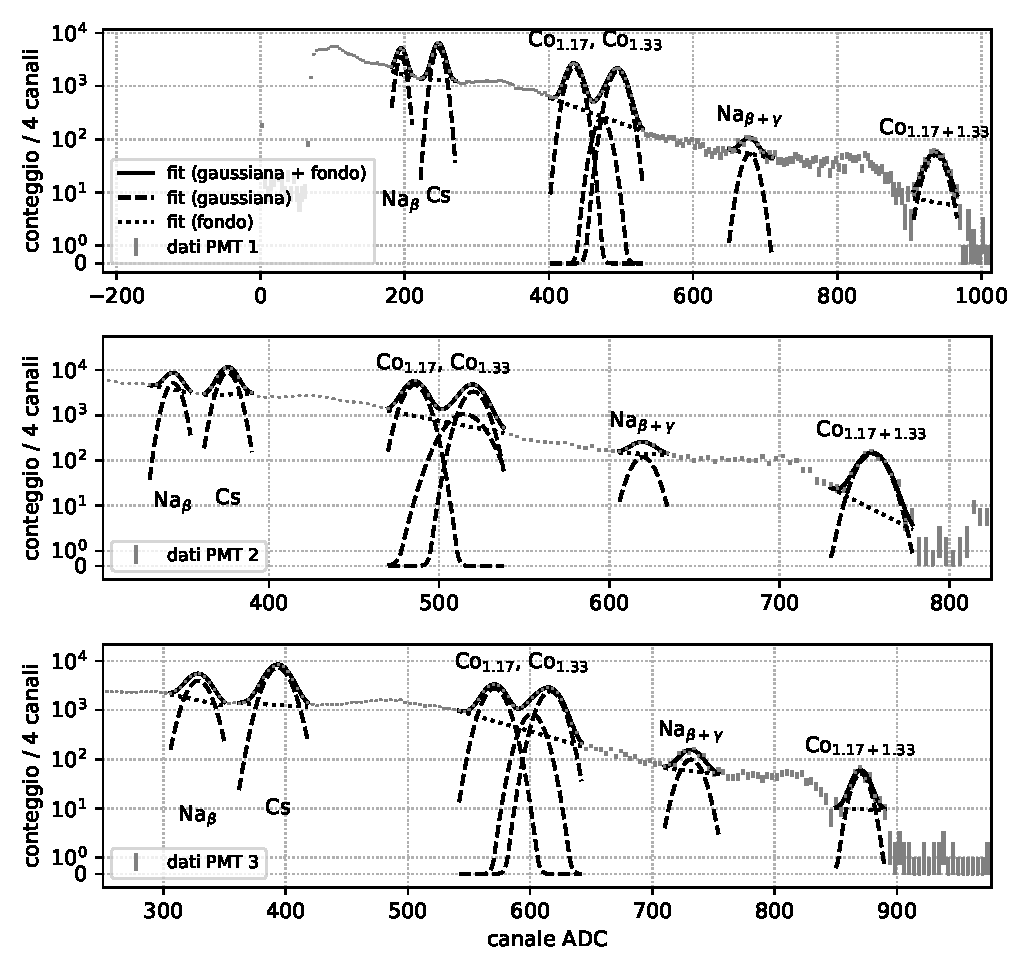
\includegraphics[width=\textwidth]{immagini/mass18-peaks}
	\caption{\label{fig:mass18-peaks}
	Spettri e fit dei picchi delle sorgenti \na{}, \cs{} e \co{} con i tre PMT,
	usati per ricavare la massa dell'elettrone,
	ovvero l'energia del picco di annichilazione $\na_\beta$.
	Nel fit dei picchi $\co_{1.17}$ e $\co_{1.33}$ c'è una terza gaussiana
	perché tra i due c'è il picco $\na_\gamma$ a \SI{1.28}{MeV},
	ma ha un rate parecchio minore quindi lo fittiamo come fondo ma non lo usiamo per ricavare la massa.
	Il picco $\na_{\beta+\gamma}$ è dovuto al caso in cui lo scintillatore
	assorbe sia il fotone dell'annichilazione sia quello del neon;
	analogamente $\co_{1.17+1.33}$ è il caso in cui vengono assorbiti entrambi i fotoni del cobalto.}
\end{figure}

Fittiamo ogni picco, scegliendo a mano l'intervallo di canali su cui fittare,
con una gaussiana più un esponenziale come fondo.
Il fit è ai minimi quadrati sull'istogramma.
I bin fittati contengono tutti almeno 5 eventi.
Controlliamo che cambiare il ribinnaggio dei canali dell'ADC non cambia significativamente il risultato.
I~fit sono riportati in \autoref{fig:mass18-peaks}.
Tutti i fit hanno un p-value ragionevole;
il test di Kolmogorov-Smirnov sull'uniformità dei p-value dà un p-value del \SI{18}\%.
Per i picchi del cobalto e quello del neon, che sono sovrapposti, il fit è unico.
Con dei test vediamo che il risultato per la media del picco del neon,
che è praticamente nascosto da quelli del cobalto,
è instabile, quindi lo teniamo nel fit come fondo ma non lo usiamo per ricavare la massa.

\subsubsection{Fit della massa}

\begin{figure}
	\centering
	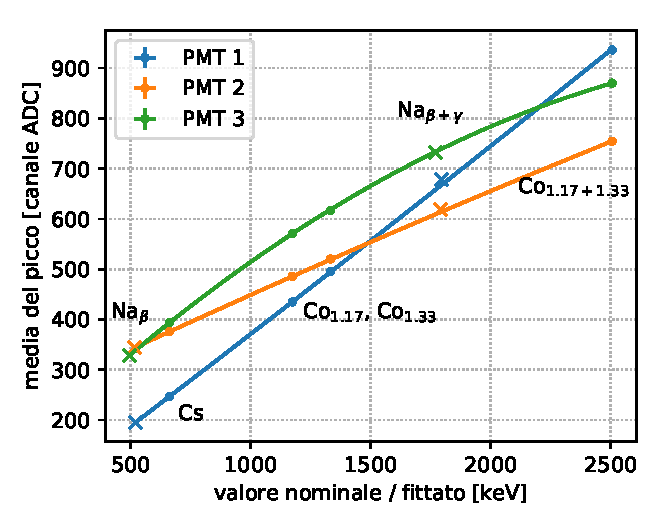
\includegraphics[width=25em]{immagini/mass18-cal}
	\caption{\label{fig:mass18-cal}
	Fit per ricavare la massa dell'elettrone.
	Sulle ordinate sono riportate le medie dei picchi di \autoref{fig:mass18-peaks}.
	Sulle ascisse sono riportati i valori noti delle energie
	per $\cs$, $\co_{1.17}$, $\co_{1.33}$, $\co_{1.17+1.33}$ (pallini),
	mentre per $\na_\beta$ e $\na_{\beta+\gamma}$ (croci) sono riportati i valori fittati.
	Le incertezze non sono visibili a questa scala.}
\end{figure}

\begin{table}
	\hspace{-3em}
	\begin{tabular}{c|cccc|cc}
		PMT & $a$ & $b$ [\si{keV^{-1}}] & $c$ [\si{keV^{-2}}] & $m$ [\si{keV}] & $\chi^2$/dof & $F$ \\
		\hline
		1 &   \num{7.31(54)} &  \num{0.3584(11)} &   \num{2.60(26)} & \num{519.95(50)} & 33.3 & 7.0 \\
		2 & \num{228.02(31)} & \num{0.22802(56)} &  \num{-3.55(11)} & \num{516.44(55)} & 24.4 & 6.2 \\
		3 & \num{113.47(44)} & \num{0.46701(84)} & \num{-32.94(18)} & \num{495.25(44)} &  4.1 & 2.2
	\end{tabular}
	\caption{\label{tab:massfit}
	Risultati dei fit di calibrazione e massa dell'elettrone per ogni PMT.
	La curva di calibrazione è $E_\text{adc}=2cE^2+bE+a$.
	In tutti i fit le correlazioni risultano circa \SI{50}\% tra $m$ e gli altri parametri
	e circa \SI{95}\% tra $a$, $b$ e $c$.
	$F$ è il fattore per cui riscalare l'incertezza su $m$
	ricavato testando il fit sui picchi di calibrazione.}
\end{table}

Inizialmente fittiamo le medie dei picchi in funzione dell'energia con una retta
\begin{equation}
	\label{eq:retta}
	E_\text{adc} = b \cdot E + a,
\end{equation}
dove, a seconda dei casi, $E$ è
\begin{itemize}
	\item il valore noto dell'energia per i picchi di calibrazione;
	\item la massa $m$ dell'elettrone (parametro di fit) per il picco di annichilazione;
	\item $m$ più l'energia del fotone del neon per il picco $\na_{\beta+\gamma}$.
\end{itemize}
Nel fit teniamo conto della correlazione tra i picchi del cobalto.
Il p-value del fit è praticamente 0,
ovvero le incertezze statistiche sono sufficientemente piccole da rigettare il modello \eqref{eq:retta}.

Poiché abbiamo ancora 3 gradi di libertà,
rendiamo il modello più generico aggiungendo il termine quadratico:
\begin{equation}
	\label{eq:parabola}
	E_\text{adc} = 2c \cdot E^2 + b \cdot E + a.
\end{equation}
Anche questo modello viene rigettato con forza per i PMT 1 e 2, ma non per il 3.
Non vogliamo avere meno di due gradi di libertà nel fit,
quindi in mancanza di un modello adeguato, stimiamo un'incertezza sistematica aggiuntiva in questo modo:
per ogni picco di calibrazione ripetiamo il fit lasciando libera,
oltre all'energia del picco di annichilazione,
anche l'energia del picco di calibrazione scelto.
Per ognuno di questi fit calcoliamo il rapporto tra
la differenza tra l'energia fittata e l'energia nota del picco di calibrazione
e la deviazione standard stimata dal fit sull'energia fittata.
Riscaliamo l'incertezza sulla massa del fit principale
per la media quadratica di questi rapporti.
Nel caso dei due picchi del cobalto $\co_{1.17}$ e $\co_{1.33}$,
per il picco $\co_{1.17+1.33}$ scriviamo $E$ come somma di un parametro di fit e di un valore noto
allo stesso modo del picco $\na_{\beta+\gamma}$.
Il grafico del fit è riportato in \autoref{fig:mass18-cal},
i risultati dettagliati sono riportati in \autoref{tab:massfit}.
Le masse fittate, con l'incertezza riscalata, risultano
\begin{center}
	\begin{tabular}{cc}
		PMT 1: & $m=\SI{520.0(35)}{keV}$, \\
		PMT 2: & $m=\SI{516.4(34)}{keV}$, \\
		PMT 3: & $m=\SI{495.2(10)}{keV}$.
	\end{tabular}
\end{center}
I risultati non sono complessivamente compatibili tra loro,
allora calcoliamo media e deviazione standard dei tre valori,
trascurando le incertezze riportate perché sono abbastanza minori della discrepanza.
Risulta $m=\SI{511(13)}{keV}$.
% Come si vede chiaramente in \autoref{fig:mass18-cal}
% il PMT 3 è molto meno lineare di 1 e 2,
% però avendo stimato l'incertezza testando il fit sui picchi di calibrazione
% non è giustificato escluderlo.

\paragraph{Instabilità della calibrazione}

Pur avendo usato tutte le sorgenti contemporaneamente,
controlliamo se l'instabilità della scala di energia ha un effetto sulla misura.
Dividendo a metà l'acquisizione e analizzando separatamente le due parti
si osserva uno spostamento visibile dei picchi ma minore della loro deviazione standard.
I due risultati per la massa, separati per rivelatore,
sono compatibili all'incertezza statistica
(dell'ordine di quella riportata in \autoref{tab:massfit}),
quindi concludiamo che l'effetto è trascurabile.
